%%%%%%%%%%%%%%%%%%%%%%%%%%%%%%%%%%%%%%%%%%%%%%%%%%%%%%%%%%%%%%%%%%%%%%%%%%%%%%%%
%2345678901234567890123456789012345678901234567890123456789012345678901234567890
%        1         2         3         4         5         6         7         8

\documentclass[letterpaper, 10 pt, conference]{ieeeconf}  % Comment this line out
                                                          % if you need a4paper
%\documentclass[a4paper, 10pt, conference]{ieeeconf}      % Use this line for a4
                                                          % paper

\IEEEoverridecommandlockouts                              % This command is only
                                                          % needed if you want to
                                                          % use the \thanks command
\overrideIEEEmargins
% See the \addtolength command later in the file to balance the column lengths
% on the last page of the document



% The following packages can be found on http:\\www.ctan.org
\usepackage{graphicx} % for pdf, bitmapped graphics files
%\usepackage{epsfig} % for postscript graphics files
\usepackage{mathptmx} % assumes new font selection scheme installed
\usepackage{times} % assumes new font selection scheme installed
%\usepackage{amsmath} % assumes amsmath package installed
%\usepackage{amssymb}  % assumes amsmath package installed

\title{\LARGE \bf
Preparation of Papers for ICCD 2008
}

%AUTHORS -- it is acceptable to add lines for affiliations (e.g., department).

\author{First Author, Second Author and Third Author% <-this % stops a space
	\\\textit{Author Affiliation}%
	\\\textit{Author Email Addresses}
}
% For authors with multiple affiliations, use multiple centered parboxes, as follows...
%\author{ \parbox{2 in}{\centering Huibert Kwakernaak\\
%         \textit{University of Twente}\\
%         \textit{h.kwakernaak@autsubmit.com}}
%         \hspace*{0.5 in}
%         \parbox{2 in}{ \centering Pradeep Misra\\
%         \textit{Wright State University}\\
%         \textit{pmisra@cs.wright.edu}}
%}
%


\begin{document}



\maketitle
\thispagestyle{empty}
\pagestyle{empty}


%%%%%%%%%%%%%%%%%%%%%%%%%%%%%%%%%%%%%%%%%%%%%%%%%%%%%%%%%%%%%%%%%%%%%%%%%%%%%%%%
\begin{abstract}

These instructions provide basic guidelines for preparing papers for submission
and for final camera-ready copy for ICCD 2008.  This document is itself an example of the
desired layout (inclusive of this abstract). The document
contains information regarding format, type sizes, and
type faces. Style rules are provided that explain how to handle equations,
units, figures, tables, references, abbreviations, and acronyms. Sections
are also devoted to the preparation of the references and acknowledgments.

\end{abstract}


%%%%%%%%%%%%%%%%%%%%%%%%%%%%%%%%%%%%%%%%%%%%%%%%%%%%%%%%%%%%%%%%%%%%%%%%%%%%%%%%
\section{Introduction}

Your goal is to simulate, as closely as possible, the usual appearance of typeset
 papers. This document provides an example of the desired layout and contains
 information regarding desktop publishing format, type sizes, and type faces.

\subsection{Full-Size Camera-Ready (CR) Copy}

Prepare your ICCD paper using letter-sized paper: 21.6 x 27.9 cm (8.5 x 11 in or 51 x 66 picas).
Create an IEEE-compliant PDF file for submission and final versions.

\addtolength{\textheight}{-3cm}   % This command serves to balance the column lengths
                                  % on the last page of the document manually. It shortens
                                  % the textheight of the last page by a suitable amount.
                                  % This command does not take effect until the next page
                                  % so it should come on the page before the last. Make
                                  % sure that you do not shorten the textheight too much.

\subsubsection{Typefaces and Sizes} Use a proportional serif typeface such as Times Roman. 
If possible, use the {\em times} and {\em mathptm} packages.
If these are not available to you, use the closest typeface you
  can. The minimum typesize for the body of the text is 10 point. The minimum
  size for applications like table captions, footnotes, and text subscripts
  is 8 point. 

\subsubsection{Margins} Set top and
bottom margins to 25 mm (1 in or 6 picas), and left and right margins
to about 18 mm (0.7 in or 4 picas). The column width is 88 mm (3.5 in or 21 picas).
 The space between the two columns is 5 mm(0.2 in or 1 pica). Paragraph
 indentation is about 3.5 mm (0.14 in or 1 pica). Left- and right-justify your
 columns. Use either one or two spaces between sections,
 and between text and tables or figures, to adjust the column length.
  On the last page of your paper, try to adjust the lengths of the
  two-columns so that they are the same. (See the source for this file 
({\em sample\_new.tex}) to see an example of setting the \\textlength 
of the last page to balance columns.)

Use automatic hyphenation and check spelling. 

\section{Section Formatting}

\subsection{Title} 

The top of the title starts 18 points below the top margin.
The text is bold, centered, and a 16-point font.  Leave a blank line between
the title and the author names.

\subsection{Authors}  

\textbf{NOTE: ICCD uses a double-blind review process.  When you submit your paper
for review, do not include author names, affiliations, or emails.  This section
{\em only} applies for the final camera-ready copy.}

Author names are in 11-point font.  Author affiliations
and email addresses are in italics, 11-point fonts, and centered beneath the names.
(Multiple lines may be used for the affiliation, if desired.)  The exact format
of the author names can be flexible, as long as the required information is provided
in the proper font size, etc.   The source file for this document ({\em sample\_new.tex}) 
shows an example of how to group authors with different affiliations.

Leave two blank lines between the authors and the abstract.

\textbf{NOTE: ICCD uses a double-blind review process.  When you submit your paper
for review, do not include author names, affiliations, or emails.  This section
{\em only} applies for the final camera-ready copy.}

\subsection{Abstract} 

The abstract is in 9-point font.  It begins with the word 
``Abstract'' in italics, followed by an em-dash.  The body of the abstract follows
in bold, 9-point type.  Multiple paragraphs must be indented, with no space
in between.

Leave one blank line between the abstract and the first section of text.


%%%%%%%%%%%%%%%%%%%%%%%%%%%%%%%%%%%%%%%%%%%%%%%%%%%%%%%%%%%%%%%%%%%%%%%%%%%%%%%%

\section{Section Numbering and Headers}

Number sections using upper-case Roman numerals.  The section heading must
be centered, on a line by itself, and in all upper-case letters in 10-point font.  
Leave at least one blank line before an after a section heading.

\subsection{Subsections}
Number subsections using upper-case letters.  For example, the first subsection of 
Section III would be labeled ``A''; a reference to that subsection from elsewhere
in the documents would be ``III.A''.  The subsection heading must be left-justified,
on a line by itself, in italics and 10-point font.  Leave at least one blank line before and after
a subsection heading.

All paragraphs within a section must be indented.  Do not leave space between
paragraphs.

\subsubsection{Sub-subsections} Sub-subsections are not recommended, but must be 
numbered using Arabic numerals, followed by a closing parenthesis.  The sub-subsection 
heading is part of the first paragraph; it is indented (just like all paragraphs), 
and the heading text must be in italics, followed by a colon.  A reference to the 
third sub-subsection of Section III.A would be ``III.A.3''.

%%%%%%%%%%%%%%%%%%%%%%%%%%%%%%%%%%%%%%%%%%%%%%%%%%%%%%%%%%%%%%%%%%%%%%%%%%%%%%%%
\section{Additional Requirements}

\subsection{Figures and Tables}

Position figures and tables at the tops and bottoms of columns.
Avoid placing them in the middle of columns. Large figures and tables
may span across both columns. Figure captions should be below the figures;
 table captions should be above the tables. Avoid placing figures and tables
  before their first mention in the text. Use the abbreviation ``Fig. 1'',
  even at the beginning of a sentence.
Figure axis labels are often a source of confusion.
Try to use words rather then symbols. As an example write the quantity ``Inductance",
 or ``Inductance L'', not just ``L''.
 Put units in parentheses. Do not label axes only with units.
 In the example, write ``Inductance (mH)'', or ``Inductance L (mH)'', not just ``mH''.
 Do not label axes with the ratio of quantities and units.
 For example, write ``Temperature (K)'', not ``Temperature/K''.

\begin{table}[t]
\caption{An Example of a Table}
\label{table_example}
\begin{center}
\begin{tabular}{|c||c|}
\hline
One & Two\\
\hline
Three & Four\\
\hline
\end{tabular}
\end{center}
\end{table}

\subsection{Citations and Reference List}

Number reference citations consecutively in square brackets \cite{IEEEexample:article_typical}.
 The sentence punctuation follows the brackets \cite{IEEEexample:articleetal}.
 Refer simply to the reference number, as in \cite{IEEEexample:conf_typical}.
 Do not use ``ref. \cite{IEEEexample:conf_typical}'' or ``reference \cite{IEEEexample:conf_typical}''.

References are important to the reader; therefore, each citation must be complete and correct. 
If at all possible, references should be commonly available publications.  References must appear in an 
unnumbered section named ''References'' at the end of the paper (before any appendices).

The {\em IEEEtrans.bst} file is provided, which is the standard BibTeX
style file for IEEE publications.  {\em IEEEexample.bib} is an example
BibTeX file that shows many types of references.  Four example references
\cite{IEEEexample:article_typical,IEEEexample:articleetal,%
IEEEexample:conf_typical,IEEEexample:book_typical} are shown at
the end of this document.


\subsection{Abbreviations and Acronyms}

Define abbreviations and acronyms the first time they are used in the text,
even after they have been defined in the abstract. Abbreviations such as
IEEE, SI, CGS, ac, dc, and rms do not have to be defined. Do not use
abbreviations in the title unless they are unavoidable.

\subsection{Equations}

Number equations consecutively with equation numbers in parentheses flush
 with the right margin, as in (1). 
Punctuate equations with commas or periods when they are part of a sentence:
\begin{equation}
\Gamma_2 a^2 + \Gamma_3 a^3 + \Gamma_4 a^4 + ... = \lambda \Lambda(x),
\end{equation}
where $\lambda$ is an auxiliary parameter.

Be sure that the symbols in your equation have been defined before the
equation appears or immediately following.
Use ``(1),'' not ``Eq. (1)'' or ``Equation (1),''
except at the beginning of a sentence: ``Equation (1) is ...''.

   \begin{figure}[tpb]
      \centering
      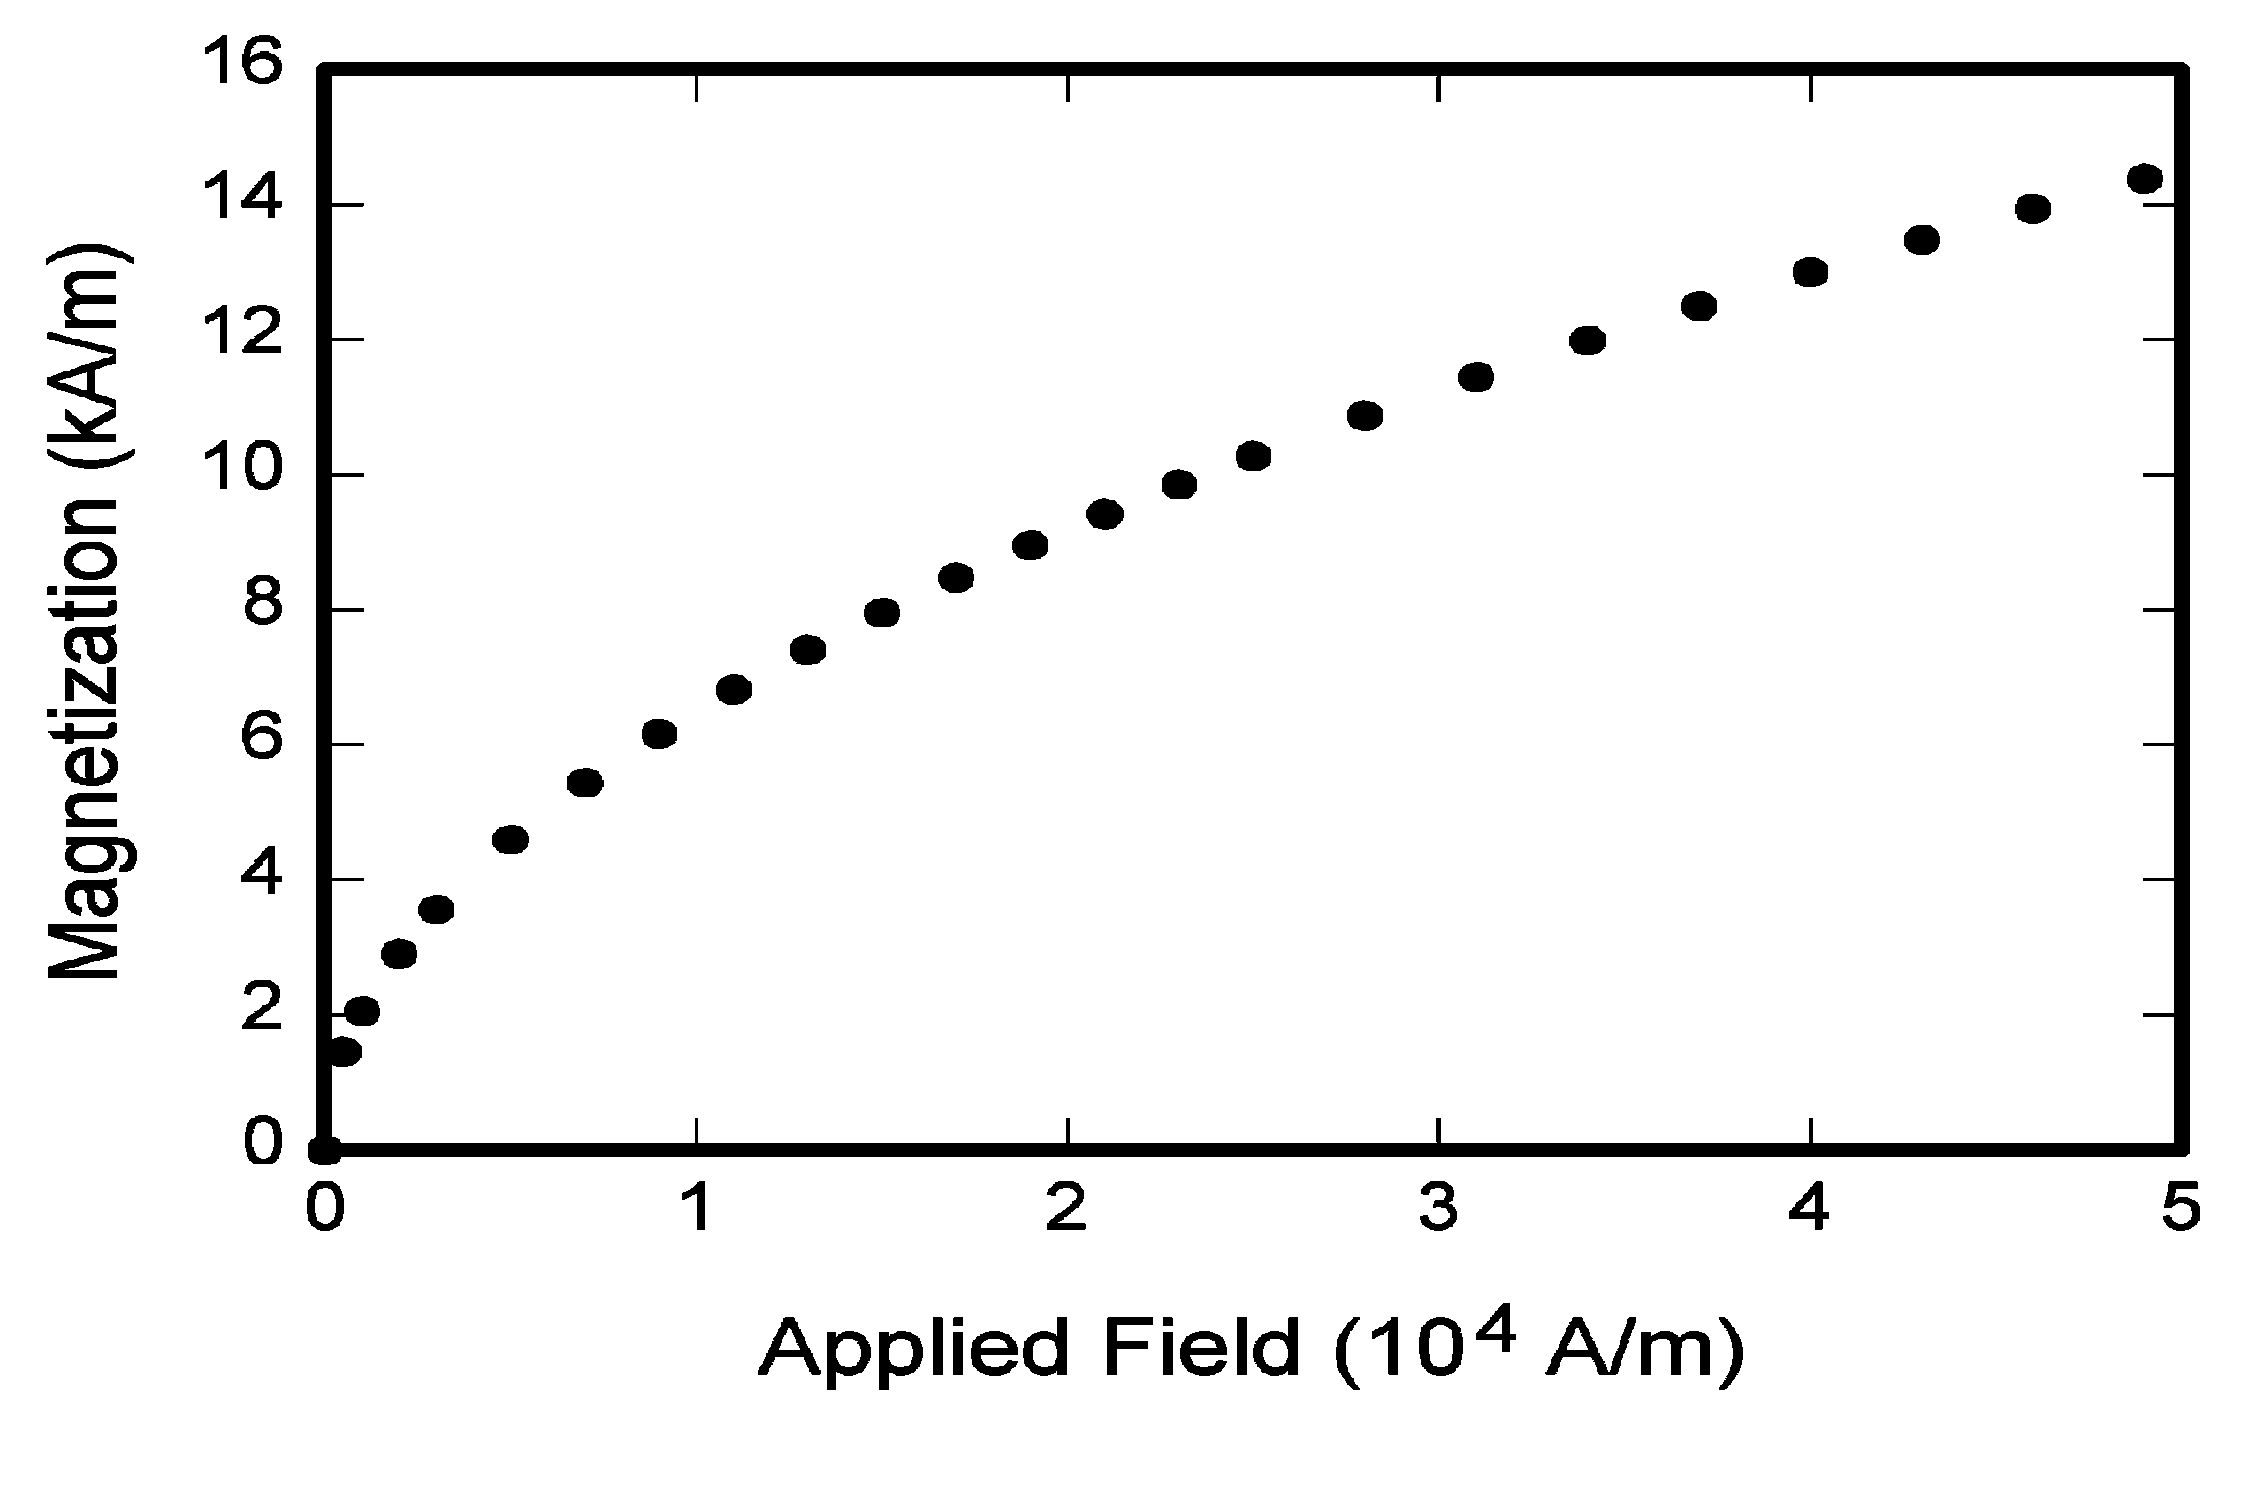
\includegraphics[width=0.9\columnwidth]{figurefile}
      \caption{Inductance of oscillation winding on amorphous
       magnetic core versus DC bias magnetic field}
      \label{figurelabel}
   \end{figure}

%%%%%%%%%%%%%%%%%%%%%%%%%%%%%%%%%%%%%%%%%%%%%%%%%%%%%%%%%%%%%%%%%%%%%%%%%%%%%%%%

%\section{Conclusions and Future Work}
%
%\subsection{Conclusions}
%
%This is a repeat.
%Position figures and tables at the tops and bottoms of columns.
%Avoid placing them in the middle of columns. Large figures and tables
%may span across both columns. Figure captions should be below the figures;
% table captions should be above the tables. Avoid placing figures and tables
%  before their first mention in the text. Use the abbreviation ``Fig. 1'',
%  even at the beginning of a sentence.
%Figure axis labels are often a source of confusion.
%Try to use words rather then symbols. As an example write the quantity ``Inductance",
% or ``Inductance L'', not just.
% Put units in parentheses. Do not label axes only with units.
% In the example, write ``Inductance (mH)'', or ``Inductance L (mH)'', not just ``mH''.
% Do not label axes with the ratio of quantities and units.
% For example, write ``Temperature (K)'', not ``Temperature/K''.
%
%
%\subsection{Future Work}
%
%This is a repeat.
%Position figures and tables at the tops and bottoms of columns.
%Avoid placing them in the middle of columns. Large figures and tables
%may span across both columns. Figure captions should be below the figures;
% table captions should be above the tables. Avoid placing figures and tables
%  before their first mention in the text. Use the abbreviation ``Fig. 1'',
%  even at the beginning of a sentence.
%Figure axis labels are often a source of confusion.
%Try to use words rather then symbols. As an example write the quantity ``Inductance",
% or ``Inductance L'', not just.
% Put units in parentheses. Do not label axes only with units.
% In the example, write ``Inductance (mH)'', or ``Inductance L (mH)'', not just ``mH''.
% Do not label axes with the ratio of quantities and units.
% For example, write ``Temperature (K)'', not ``Temperature/K''.
%
%%%%%%%%%%%%%%%%%%%%%%%%%%%%%%%%%%%%%%%%%%%%%%%%%%%%%%%%%%%%%%%%%%%%%%%%%%%%%%%%
\section{Acknowledgments}

The authors gratefully acknowledge the contribution of National Research Organization and reviewers' comments.


%%%%%%%%%%%%%%%%%%%%%%%%%%%%%%%%%%%%%%%%%%%%%%%%%%%%%%%%%%%%%%%%%%%%%%%%%%%%%%%%

\bibliographystyle{IEEEtran}
\bibliography{IEEEabrv,IEEEexample}


%\begin{thebibliography}{99}
%
%\bibitem{c1}
%J.G.F. Francis, The QR Transformation I, {\it Comput. J.}, vol. 4, 1961, pp 265-271.
%
%\bibitem{c2}
%H. Kwakernaak and R. Sivan, {\it Modern Signals and Systems}, Prentice Hall, Englewood Cliffs, NJ; 1991.
%
%\bibitem{c3}
%D. Boley and R. Maier, "A Parallel QR Algorithm for the Non-Symmetric Eigenvalue Algorithm", {\it in Third SIAM Conference on Applied Linear Algebra}, Madison, WI, 1988, pp. A20.
%
%\end{thebibliography}

\end{document}
